\section{Ukázky}

\subsection{Spuštění instance systému}

Ukázka \ref{fig:openstack} zobrazuje proces spouštění nové instance systému v cloudovém prostředí OpenStack \cite{openstack}.
Uživatel pomocí průvodce přidělí systémové prostředky a zvolí požadovanou konfiguraci systému.
Průvodce nabízí uživateli možnost vložit skript, který nastaví potřebná data pro inicializaci a umožní automatickou instalaci herního serveru. 

\begin{figure}[h]
    \centering
    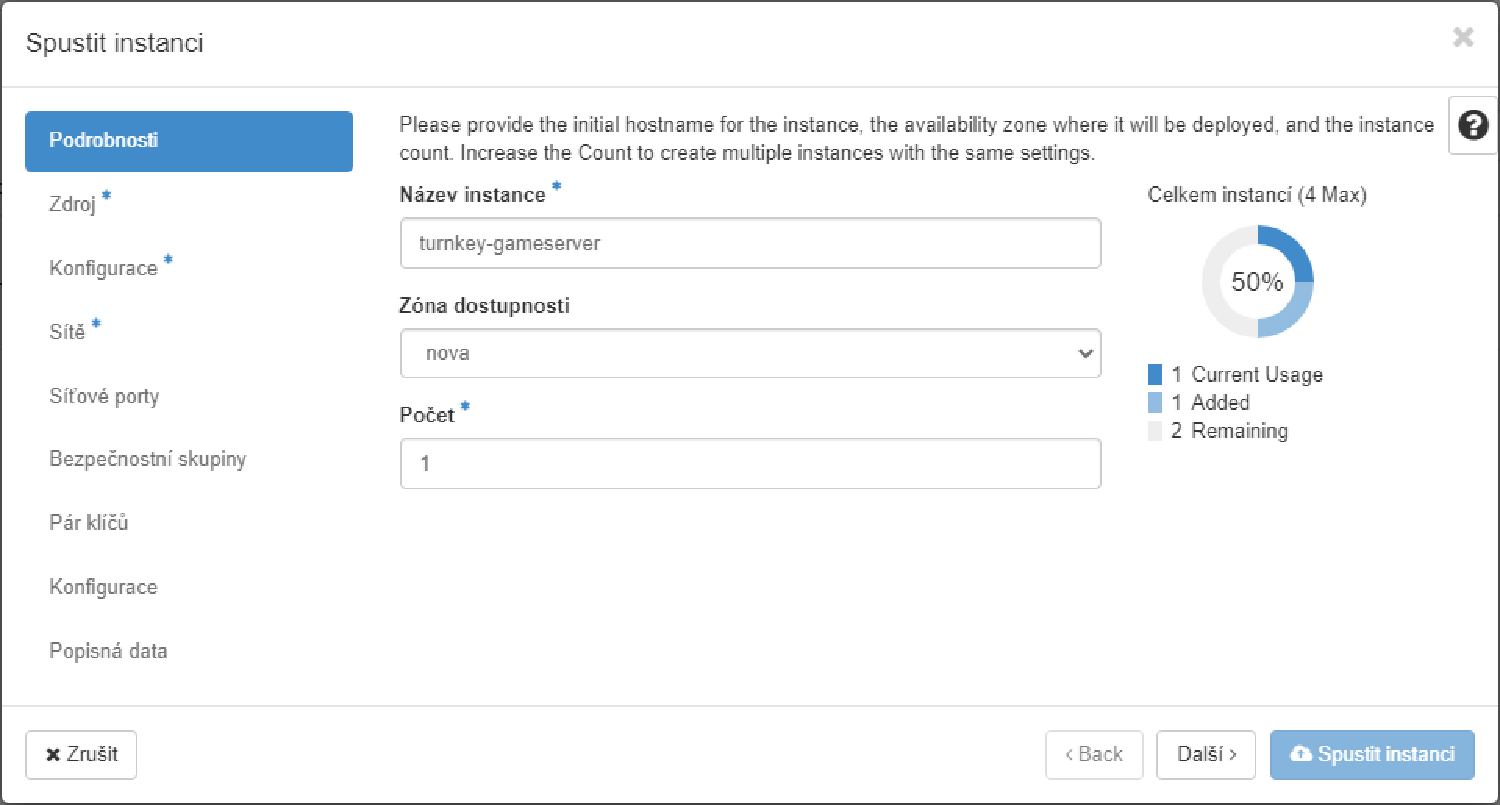
\includegraphics[width=1\linewidth]{chapters/images/openstack.pdf}
    \caption{Spuštění systému v prostředí OpenStack \cite{openstack}}
    \label{fig:openstack}
\end{figure}

\subsection{Interaktivní výběr herního serveru}

Na obrázku \ref{fig:game-selection} je zobrazen interaktivní výběr herního serveru. Tento výběr je automaticky
k dispozici při prvním spuštění systému, pokud uživatel neurčil herní server pomocí inicializačního skriptu.

\begin{figure}[h]
    \centering
    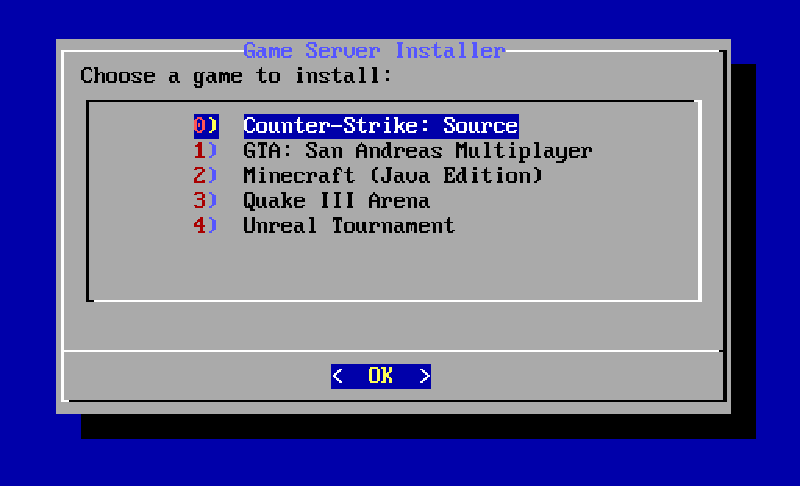
\includegraphics[width=1\linewidth]{chapters/images/game-selection.pdf}
    \caption{Interaktivní výběr hry při prvním spuštění}
    \label{fig:game-selection}
\end{figure}

\subsection{Automatický výběr herního serveru}

V případě plně automatického nasazení herního serveru je nutné použít inicializační skript, který před prvním spuštěním systému
zapíše do souboru \mintinline{shell}{/etc/inithooks.conf} potřebná data pro automatickou konfiguraci systému.
V ukázce \ref{code:init-script} je uveden inicializační skript, pomocí kterého dojde k instalaci herního serveru pro hru \mintinline{shell}{GTA: San Andreas Multiplayer}
včetně nastavení administrátora serveru.

\begin{listing}[h!]
    \caption{Ukázkový inicializační skript}
    \label{code:init-script}
    \begin{minted}{shell}
#!/bin/bash

cat>/etc/inithooks.conf<<EOF
export ROOT_PASS=SecretRootPassword
export DB_PASS=SecretMysqlPassword
export APP_PASS=SecretGameuserPassword
export APP_EMAIL=admin@example.com
export HUB_APIKEY=SKIP
export SEC_UPDATES=FORCE

export GAME=samp
export GAME_RCON_PASS=GameserverAdminPassword
EOF
    \end{minted}
\end{listing}

\subsection{Přidání nové hry}

Ukázky \ref{code:game-props-script} a \ref{code:game-config-script} demonstrují přidání podpory pro nový herní server. Jedná se o dva skripty správce herních serverů,
které zavádějí podporu pro server hry \mintinline{shell}{Minecraft} a umožňují jeho minimální počáteční konfiguraci.
Skript \mintinline{shell}{game_properties.sh} zavádí proměnné, které jsou instalačním programem využity k identifikaci herního serveru.
Druhý skript poté umožňuje nastavit uživatelské jméno administrátora serveru pomocí předdefinované proměnné, případně interaktivně.

\begin{listing}[h]
    \caption{Skript \mintinline{shell}{game_properties.sh}}
    \label{code:game-props-script}
    \begin{minted}{shell}
GAME="mc"
GAME_LONG_NAME="Minecraft (Java Edition)"
    \end{minted}
\end{listing}

\begin{listing}[h]
    \caption{Skript \mintinline{shell}{post_install.sh}}
    \label{code:game-config-script}
    \begin{minted}{shell}
#!/bin/bash

# Set server admin
if [ -z "$GAME_ADMIN" ]; then
    read -p "Server admin username: " GAME_ADMIN || GAME_ADMIN=''
    echo
fi
run_as_user "echo \"$GAME_ADMIN\" > \"$GAMEDIR/serverfiles/ops.txt\""
    \end{minted}
\end{listing}
